%Andr� Fernandes dos Santos
%LEI, n�49344

\documentclass{article}
\usepackage[portuguese,english]{babel}
%\usepackage[utf8]{inputenc}
\usepackage[T1]{fontenc}
\usepackage{a4wide}
\usepackage{txfonts}% use Arial && Times New Roman
\usepackage[pdftex]{color,graphicx}
\usepackage{fancyhdr}
\usepackage{fancyvrb}
\usepackage{cite}
\usepackage{longtable}
\usepackage{verbatim}
\usepackage{ae}
\usepackage{multicol}
\usepackage{graphicx}

\renewcommand\familydefault{\sfdefault}% usar font sem serifas
\renewcommand{\labelitemi}{$-$}
\author{Andr� Fernandes dos Santos}
\title{Curriculum Vit\ae}
\date{\today}

\begin{document}
\maketitle
\thispagestyle{empty}

\newpage
\section{Personal Information}
	\begin{description}
	%\item [Nome:] \framebox{\textsc{Andr� Fernandes dos Santos}}
	\item [Name:] \textbf{\textsc{Andr� Fernandes dos Santos}}
	\item [Birthdate:] 24 February 1988
	\item [Address:] Pq. Resid. Fonte Seca, Lt8B 1$\,^{\circ}$E, 4715-229 BRAGA
	\item [Civil state:] Single
	\item [Mobile number:] +351 92 7715379
	\item [Email:] pg15973@alunos.uminho.pt
	\end{description}

%	\begin{figure}[htbp]
%	\centering
%	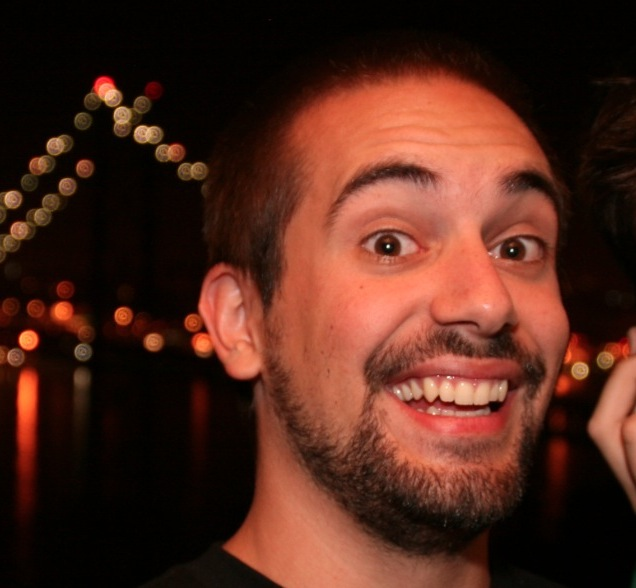
\includegraphics[width=.1\textwidth]{foto}
%	\end{figure}

\section{Education}
\begin{description}
\item [2006-2009] Degree in Software Engineering, University of Minho (final grade 14.56/20.00)
\item [2009/2010] 1${^\textrm{st}}$ year of Software Engineering MSc, University of Minho
	\begin{itemize}
		\item Languages Engineering
		\item Bioinformatics
	\end{itemize}
\item [2010/present] 2${^\textrm{st}}$ year of Software Engineering MSc, University of Minho
	\begin{itemize}
		\item Master thesis: ``Building a Corpora-Flow System''
	\end{itemize}
\end{description}

\section {Training}
\begin {description}
\item [Jul 2005] German Open Course, U. Junior, Faculty of Arts, University of Porto
\item [Set 2005] Physics Summer School, Faculty of Science, University of Porto
\item [Jun 2010] Catalyst 5.80 (\textit{Portuguese Perl Workshop 2010}, Porto)
\item [Jul 2010] Escola de Computa��o Evolutiva (UMinho, Guimar�es)
\end{description}

\section{Professional Experience}
\begin{description}
\item [Jul-Set 2009] Traineeship Sapo Summerbits 2009
\end{description}

\section{Technical Skills}
\begin{description}
\item[-] Experience with PASCAL, C\#, PHP, JavaScript, UML, XML, Html, SQL, Haskell;
\item[-] Proficiency with C, Java and Perl;
\item[-] Unix sys admin experience
\item[-] Others: \LaTeX, bash, Subversion, Git, Apache and associated technologies.
\end{description}

\section{Other Activities}
\begin{description}
\item [1999-2011] Judo, 4$\,^{\textrm{th}}$~Kyu
\item [Out 2007] Inter-University Programming Marathon (IST, UTL, Lisbon)
\item [Out 2008] Inter-University Programming Marathon (UC, Coimbra)
\item [Nov 2008] ACM South Western European Regional Contests (Nuremberg, Germany)
\item [Out 2009] Inter-University Programming Marathon (ESTGA, Aveiro)
\item [2008-2011] Member of CeSIUM (UMinho's Software Engineering Student Center)
\item [2009/2010] Vice-President of CeSIUM 
\item [2010/2011] Director of CAOS (Open Source Support Center)
\end{description}

\renewcommand*{\refname}{}
\section{Publications}
\bibliographystyle{plain}
\bibliography{aspubs}
\nocite{*}

\end{document}

